\documentclass{article}

\usepackage{tikz}
\usetikzlibrary{bayesnet}
\usepackage{tikz-3dplot} 
%\usetikzlibrary{arrows,decorations.pathmorphing,fit,positioning}

\usetikzlibrary{positioning, shapes.geometric}
% \newcommand{\semaphore}[4]{% #1: color of circle, 
%                            % #2: color of semicircle
%                            % #3: angle of semicircle 
% \tikz[node distance=0mm,baseline]
%     {
%     \node (#1) [circle, fill=draw=black,inner sep=1pt,minimum size=20pt, font=\fontsize{10}{10}\selectfont, node distance=1] {#2};
%     \node      [semicircle, fill=#3, 
%                 inner sep=0pt, outer sep=0pt, minimum size=18pt,
%                 anchor=south,
%                 at={(#1.center)}, rotate=#4] {};
%      }
%                         }% end of command


\newcommand{\bs}[1]{\ensuremath{\mathbf{x}}}

\begin{document}



\begin{center}
  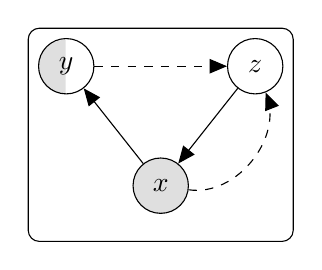
\begin{tikzpicture}

    \node[obs](x){$x$};
  \node[latent, above=0.8cm of x, xshift=1.2cm](z){$z$};
  \node(s2) [semicircle, fill=gray!25, 
                inner sep=1pt, minimum size=9.8pt,
                node distance=1,
                anchor=south,
                % at={(y.center)},
                above=1.15cm of x, xshift=-1.2cm,
                rotate=90] {};
  \node[latent,fill=none, above=0.8cm of x, xshift=-1.2cm] (y) {$y$};

  \plate {xyz} {(x) (y) (z) (s2)} {} ;

  \edge {z} {x}
  \edge {x} {y}
  \edge[dashed]{y}{z}

  \path[->,dashed] (x) edge [bend right=60] (z);

\end{tikzpicture}
\end{center}

\end{document}